\documentclass[12pt,a4paper]{article}

\usepackage{style2017}
\newcounter{numexo}
\setcellgapes{1pt}

\begin{document}


\begin{NSI}
{Activité}{Le protocole HTTP}
\end{NSI}

\section{Introduction}

Le \textbf{web} est un ensemble de serveurs sur internet proposant des contenus disponibles sous forme de page écrites au format \textbf{html}. Ces pages contiennent du texte, des images, des médias et permettent aussi d'envoyer et récupérer des données. \medskip

Pour accéder à ces multiples ressources, il est nécessaire d'utiliser des logiciels appelés navigateurs qui établissent une communication avec les serveurs disposant des contenus souhaités.

Comme dans toute communication, des règles sont nécessaires pour assurer l'envoie et la réception des données. Ces règles sont réunies dans un protocole.

Le protocole utilisé pour le web est le protocole HTTP et s'effectue dans un \textbf{modèle} dit \textbf{client - serveur}. 

\begin{center}
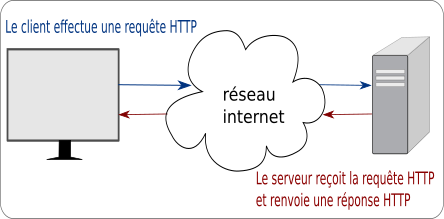
\includegraphics[scale=0.7]{img/client-serveur.eps}
\end{center}

Ce protocole permet la communication entre 2 machines, l'une étant le client et l'autre le serveur:

\begin{itemize}[label=\textbullet]
\item Le client initie la communication en réalisant une \textbf{requête} en envoyant au serveur un message.
\item Le serveur reçoit la requête et envoie au client une \textbf{réponse} quel que soit son contenu.
\end{itemize}

\noindent Une \textbf{requête HTTP} se compose des éléments suivants:
\begin{itemize}[label=\textbullet]
\item La méthode utilisée, 
\item la ressource souhaitée, 
\item le protocole utilisé et sa version
\item le destinataire de la requête.
\end{itemize}\medskip

\noindent Le serveur répond toujours à une requête HTTP qu'il reçoit. La \textbf{réponse HTTP} se compose (selon la requête) des éléments suivants:

\begin{itemize}
\item Le protocole et sa version,
\item le code d'état ou de statut HTTP;
\item Le contenu de la ressource demandée. Elle peut être envoyée en plusieurs fois si celle-ci est très volumineuse.
\end{itemize}


\newpage
\section{Protocole HTTP}

\subsection*{Mise en place du protocole}
\noindent Avec le logiciel \textbf{filius}, on va créer une liaison entre un client et un serveur web et observer les échanges entre les deux machines.\medskip

Lancez le logiciel puis:
\begin{enumerate}
\item créer une communication entre un portable (client) et un ordinateur (serveur).
\item ajouter un serveur web et le démarrer.
\item ajouter un navigateur web sur le client et afficher la page web du serveur.
\item Afficher la table d'échanges de données du client ou du serveur.
\end{enumerate}


\subsection*{Analyse du protocole}

\begin{enumerate}
\item Dans la table d'échanges du client, affichez la ligne qui initie la requête HTTP puis relevez les informations de la requête.
\vspace{5cm}

\item Dans la table d'échanges du serveur, affichez la première ligne qui contient la réponse du serveur au client puis relevez les information contenues dans la réponse.
\vspace{5cm}

\item Une autre requête HTTP a été envoyée par le client. Pourquoi ? 
\vspace{2cm}

\item Quelles sont les informations contenues dans la seconde requête HTTP ?
\vspace{4cm}

\newpage
\item La seconde requête HTTP est parvenue au serveur. Quelle est la réponse du serveur ?
\vspace{6cm}


\item Dans le navigateur du client saisir à la fin de l'url \textsf{page2}.
\begin{enumerate}
\item Qu'affiche le navigateur et pourquoi ?\vspace{1cm}
\item Quel est le contenu de la requête HTTP ? \vspace{1cm}
\item Quel est le contenu de la réponse HTTP ? \vspace{3cm}
\end{enumerate}


\end{enumerate}
%
%\newpage
%\section{Exemple réel de requête HTTP}
%
%%La manière la plus simple d'effectuer une requête HTTP est d'utiliser un navigateur comme firefox ou chrome. Ces logiciels affichent des contenus du web en utilisant le protocole HTTP ou HTTPS (protocole HTTP et le protocole TLS de sécurisation des données).
%%
%%La donnée qui permet au navigateur d'effectuer une requête HTTP  est une url que l'on saisit dans la barre d'adresse.
%%
%%Le navigateur ajoute une méthode et des informations regroupées dans l'en-tête de la requête. Elles ne sont pas directement visibles. Il est possible de les voir avec les outils de développement proposés par le navigateur. On y accède par le menu ou la touche F12 dans l'onglet \textbf{Réseau}.
%
%\subsection*{Une page web}
%Ouvrir le navigateur firefox et saisir l'url \textbf{interstices.info} puis taper sur la touche F12.\medskip
%
%Le chargement de la page d'accueil du site nous donne plusieurs informations. On remarque que l'on demande une ressource via une requête HTTP et qu'au final plusieurs requêtes HTTP ont été effectuées.
%\begin{enumerate}
%\item Combien de requêtes HTTP ont été effectuées par le navigateur ?
%\item Quelle a été la ou les méthodes employées pour ces requêtes HTTP ?
%\item Quels sont les différents codes d'état des différentes réponses HTTP ?
%\item Quels sont les différents types de contenus renvoyés par le serveur ?
%\item Certains fichiers sont transférés d'autres non. Pourquoi ? Expliquer ce que fait le navigateur.
%\item Cocher l'option \textbf{Désactiver le cache} puis recharger la page. Quelles différences a-t-on ?
%\end{enumerate}
%
%\subsection*{Requête et réponse en détail}
%
%Pour recharger une page, il suffit d'appuyer sur la touche F5 ou cliquer sur le bouton actualiser.
%
%On \textbf{sélectionne la première ligne}, celle correspondant à la requête initiale pour afficher la page d'accueil.
%
%La fenêtre est divisée en deux. À droite, on remarque différents onglets dont les en-têtes.
%
%\begin{enumerate}
%\item Quelle est la requête HTTP ? Quelles informations contient l'en-tête de la requête ?
%\item Quelle est la réponse HTTP ? Quelles informations contient l'en-tête de la réponse ?
%\item Cliquer sur le bouton \textbf{Renvoyer} puis sur \textbf{Modifier et renvoyer}. La requête HTTP est affichée.
%\begin{enumerate}
%\item Ajouter dans l'url, le mot "dossier" puis cliquer sur le bouton \textbf{Envoyer}. Sélectionner dans la liste votre requête et vérifier son code d'état et afficher l'aperçu de la réponse. 
%\item Remplacer dans l'url, le mot "dossier" par le mot "domaine" puis cliquer sur le bouton \textbf{Envoyer}. Sélectionner dans la liste votre requête et vérifier son code d'état et afficher l'aperçu de la réponse.
%\item Ajouter à l'url précédente, le mot "algorithmes" puis cliquer sur le bouton \textbf{Envoyer}. Sélectionner dans la liste votre requête et vérifier son code d'état et afficher l'aperçu de la réponse.
%\end{enumerate}
%\item Dans l'onglet \textbf{Réponse}, sélectionner \textbf{Charge utile de la réponse} (sous l'aperçu). Quel est le type de contenu ? 
%\end{enumerate}
%
%\newpage
%\section{Requêtes HTTP et paramètres}
%
%Une requête peut contenir des valeurs que l'on passe en paramètre dans l'url. Le serveur récupère les valeurs et constitue une réponse en fonction de ces paramètres. Bien entendu, ces paramètres sont connus du serveur au préalable.
%
%\subsection*{Requête de recherche textuelle}
%Sur la page d'accueil du site \textbf{Interstices.info}, vous avez dans le menu une zone de recherche matérialisée par une loupe.
%\begin{enumerate}
%\item Saisir le mot \textbf{requête} dans la zone de recherche puis valider. Quel est l'ordre chronologique ?
%\item Que remarquez-vous dans l'url ? Quelle syntaxe est utilisée pour passer le paramètre de recherche et la valeur du mot \textbf{requête}?
%\item Quelle est la méthode utilisée pour la requête HTTP lors de cette recherche ?
%\item Dans la fenêtre de développement (F12), modifier la requête HTTP en remplaçant le mot \textbf{requête} par le mot \textbf{secret} puis vérifier son aperçu dans l'onglet \textbf{Réponse}.
%\item Renvoyer une requête HTTP pour afficher les résultats par ordre chronologique croissant ?
%\item Que contient l'onglet \textbf{Requête}?
%\end{enumerate}
%
%\subsection*{Requête de recherche multiple et thématique}
%
%Sur la page d'accueil du site \textbf{Interstices.info}, vous avez une zone de recherche thématique : par domaine, par type de contenu, par niveau de lecture et chronologique.
%
%\begin{enumerate}
%\item Sélectionner pour chaque thème une valeur et observer l'url dans la barre d'adresse. Que se passe-t-il ?
%\item Quelle syntaxe est utilisée dans l'url ?
%\item Avec l'outil de développement (F12), donner la méthode employée par la requête HTTP ?
%\item La réponse envoyée par le serveur modifie directement la page web.
%\begin{enumerate}
%\item Quel est le type de ressource envoyée par le serveur ?
%\item Quel est le contenu de l'onglet \textbf{Requête} ?
%\end{enumerate}
%\item Sélectionner la requête pour la modifier en remplaçant les valeurs des paramètres. Renvoyer la requête avec les nouvelles valeurs. Quel est le code d'état de la nouvelle requête ?
%\item Effectuer une nouvelle recherche thématique. Aller sur la fenêtre de modification de la requête et effacer la partie paramètre de l'url et renvoyer la requête. Expliquer le succès de cette requête.
%\end{enumerate}
\end{document}

